\documentclass{article}
\usepackage[T1]{fontenc}
\usepackage{lmodern}
\usepackage{graphicx}
\usepackage{amsmath,amssymb}
\usepackage[a4paper,margin=2cm]{geometry}
\usepackage[absolute,overlay]{textpos}
\setlength{\TPHorizModule}{1mm}
\setlength{\TPVertModule}{1mm}
\usepackage[indonesian]{babel}
\usepackage{hyperref}
\setlength{\emergencystretch}{2em}
% unit: Halaman 3

\begin{document}

% === Halaman 3 (python/native) ===

• Algoritma ini didasarkan pada persoalan Knapsack Problem:

 Diberikan bobot knapsack adalah M. Diketahui n buah objek

 yang masing-masing bobotnya adalah w1, w2, …, wn. Tentukan nilai bi sedemikian 

sehingga


M = b1w1 + b2w2 + … + bnwn  



(1)

 yang dalam hal ini, bi bernilai 0 atau 1. Jika bi = 1, berarti objek i dimasukkan ke 

dalam knapsack, sebaliknya jika bi = 0, objek i tidak dimasukkan.

3

% deskripsi: gambar native xref 44
\noindent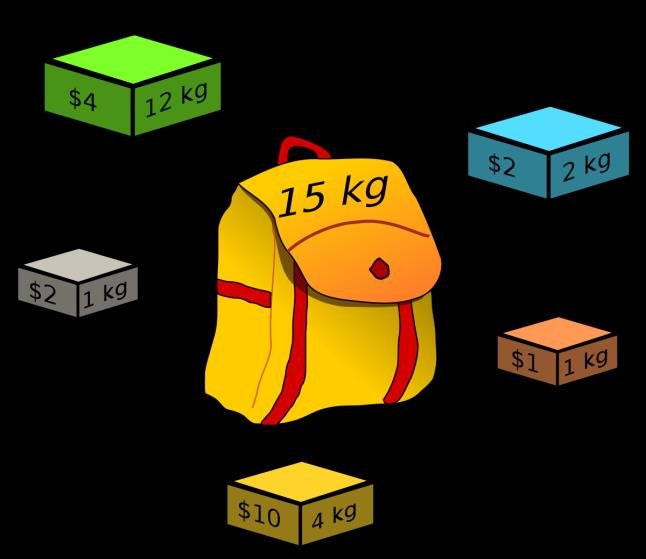
\includegraphics[width=0.85\textwidth]{../../images/python/page_003_img_01.jpeg}

\end{document}
